A common methodology is used across all three problems: Lights Out, Sudoku, and Wave Function Collapse (WFC), to ensure fair and consistent comparison. Each problem is formulated as a Boolean search problem, where candidate solutions are mapped to computational basis states of a quantum register. A reversible oracle $U_f$ is constructed to evaluate the problem constraints and mark valid solutions by applying a phase flip.

\vspace{1em}
\noindent
Figure~\ref{fig:grover_circuit} shows the general structure of a Grover iteration used throughout this work. The data qubits are initialized in the $\lvert 0 \rangle$ state and transformed into a uniform superposition using Hadamard gates. An ancilla qubit, initialized in the $\lvert 1 \rangle$ state and placed into superposition, enables phase kickback. The oracle $U_f$ marks valid solutions, after which the diffusion operator $D$ performs an inversion about the mean, amplifying the probability of measuring marked states.

\vspace{1em}
\begin{figure}[h]
    \centering
    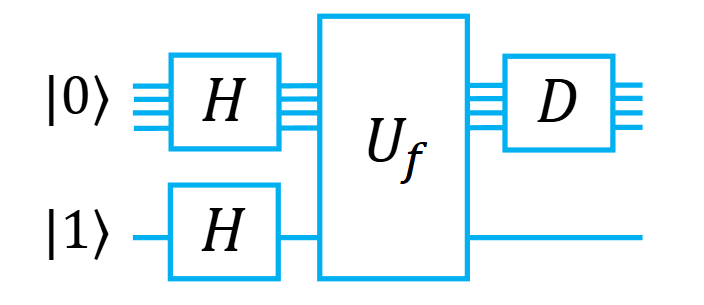
\includegraphics[width=0.8\linewidth]{figures/extra/Schermafbeelding 2026-01-24 222110.png}
    \caption{General circuit structure of Grover’s algorithm, consisting of state preparation, oracle evaluation, and diffusion \cite{BoscoLecture5}.}
    \label{fig:grover_circuit}
\end{figure}


\noindent
Oracle construction is achieved by translating classical constraint checks into reversible quantum logic. Boolean conditions are implemented using combinations of CNOT and multi-controlled gates, allowing the oracle to evaluate whether a candidate solution satisfies all required constraints. Ancilla qubits are used to store intermediate results during constraint evaluation and are uncomputed where possible to preserve reversibility and avoid residual entanglement.

\vspace{1em}
\noindent
The number of Grover iterations is chosen according to the theoretical optimum, approximately $\frac{\pi}{4}\sqrt{N/M}$, where $N$ denotes the search space size and $M$ the number of valid solutions. After the final iteration, the data qubits are measured in the computational basis.

\vspace{1em}
\noindent
All quantum circuits are implemented using Qiskit. Simulations are performed with Qiskit Aer, while selected small instances are executed on IBM quantum hardware. For each experiment, the number of qubits, transpiled circuit depth, gate counts, number of shots, success probability, and total runtime are recorded. These results form the basis for the performance analysis presented in the Results section.